\documentclass{article}
\usepackage[utf8]{inputenc}
\usepackage{enumerate}
\usepackage{enumitem}
\usepackage{float}
\usepackage{graphicx}
\usepackage{multirow, array}
\usepackage[spanish,activeacute]{babel}


\title{Práctica 2: Gestión de una Web de cine}
\author{Rafael Nogales Vaquero
\\Lothar Soto Palma
\\Elena Toro Pérez
\\Jose Ramón Trillo Vilchez}
\date{\today}

\begin{document}
\maketitle
\section{Driagramas de Conceptos}
	\subsection*{Gestión de usuarios}
	\subsection*{Gestión de películas}
	\subsection*{Gestión de cartelera}
	\subsection*{Gestión de Perfil}
	\subsection*{Gestión de películas por usuarios}
	\textbf{Problema:} Los \textbf{usuarios} podrán buscar \textbf{películas} en el sistema además de consultar la \textbf{cartelera} de \textbf{Cines}, solo si están \textbf{registrados} podrán puntuarla y tan solo los \textbf{usuarios VIP} podrán añadir y criticar películas.\\
	\textbf{Conceptos:} Usuario, Usuario registrado, Usuario VIP, Cines, Películas, Cartelera.\\
	Relaciones:
		\begin{itemize}
			\item Un cine tiene una cartelera.
			\item Todos los usuarios buscan películas.
			\item Todos los usuarios consultan la cartelera.
			\item Los registrados y los VIP pueden puntuar las películas.
			\item Los VIP pueden criticar y añadir películas.		
		\end{itemize}
		\begin{figure*}[tbph]
			\centering
			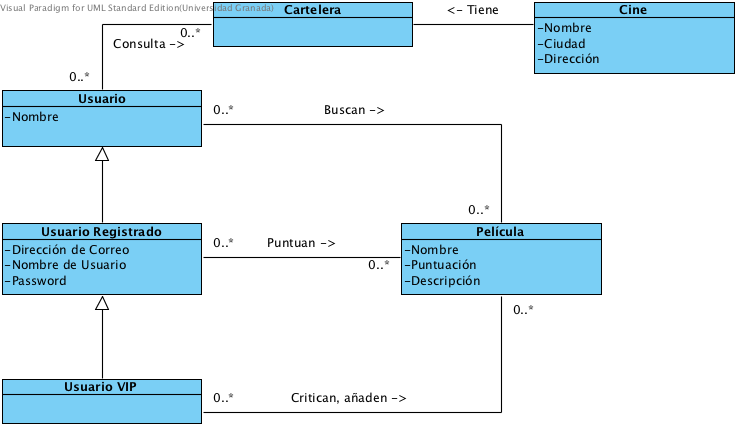
\includegraphics[width=0.9\linewidth]{./C-PeliculasUsuarios}\\
			Gestión de peliculas por usuarios.
		\end{figure*}
	\subsection*{Gestión de comunidades}
\section{Driagramas de Secuencia}
	\subsection*{Gestión de usuarios}
	\subsection*{Gestión de películas}
	\subsection*{Gestión de cartelera}
	\subsection*{Gestión de Perfil}
	\subsection*{Gestión de películas por usuarios}
	\subsection*{Gestión de comunidades}
\end{document}
